\section{TESTING ONLY}

\subsection{Achieving Ideal Load Balancing by Automatic Matrix Partitioning}

The performance analyses conducted in subsection \ref{sec:speedup} relied on perfect load balancing and thus a load balancing efficiency of \(100\%\). However, in practice achieving ideal load balancing may be difficult, because of local refinement strategies or an unfavorable grid blocking, i.e. the partition of the solution domain into grid blocks, that lead to an imbalance of load that is distributed among the involved processes. 

One possibility partially to address load imbalances is motivated by the fact, that solution algorithms which solve partial differential equations spend a significant amount of their time solving linear algebraic systems. Figures \ref{fig:distseg} and \ref{fig:distcpld} show, that approximately \(50\%\) of the wall-clock time of the segregated SIMPLE-solution algorithm, and up-to \(89\%\) of wall clock time of the coupled solution algorithm are spent solving linear systems. The goal of this subsection is to present a simple method by which ideal load balancing with respect to the linear equation solver can be obtained by automatic matrix partitioning.

The formula PETSc uses to evenly distribute vector or matrix objects containing \(N\) rows across \(m\) involved processes reads for the \(p\)th process
\begin{displaymath}
n(p)
=
\left\{\begin{array}{ll} 
    \operatorname{floor}(N/m) + 1, & \text{if} \quad  N \mod m > p \\
    \operatorname{floor}(N/m) , & \text{else}
\end{array}\right.
,
\end{displaymath}
where \(p = 0,\dots,m-1\).

Unknowns
A random number generator was used to create different grid resolutions for each one of the eight block of a block structured grid consisting of 826891 cells. Figure \ref{fig:barbalance} shows the initial distribution of unknowns and the balanced number of unknowns with respect to the matrix.
\begin{figure}[h!]
  \centering
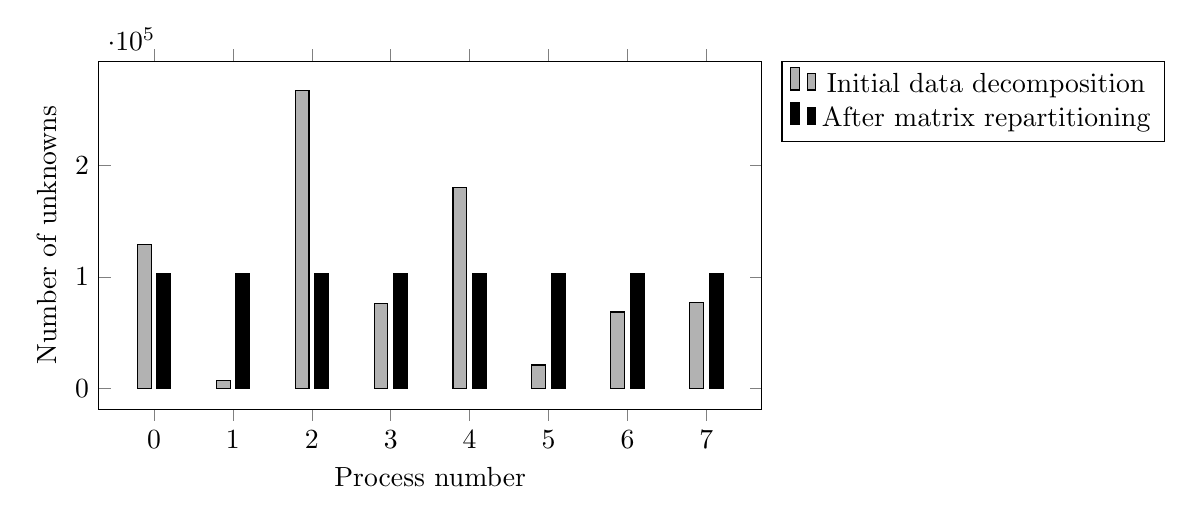
\begin{tikzpicture}
  \begin{axis}[
      %x tick label style={ /pgf/number format/1000 sep=},
      xtick={0,1,2,3,4,5,6,7},
      xlabel=Process number,
      ylabel=Number of unknowns,
      %enlargelimits=0.35,
      legend pos=outer north east,
      ybar,
      bar width=5pt,
      height=6cm,
      width=10cm
    ]
    \addplot[black,fill=black!30] coordinates {(0,129360) (1,7560) (2,267300) (3,76380) (4,179962) (5,21060) (6,68544) (7,76725)};
    \addplot[fill=black] coordinates { (0,103362) (1,103362) (2,103362) (3,103361) (4,103361) (5,103361) (6,103361) (7,103361)};
    \addlegendentry{Initial data decomposition};
    \addlegendentry{After matrix repartitioning}
  \end{axis}
\end{tikzpicture}
\caption{Comparison of the number of unknowns assigned to each process and the assigned rows of the matrix using automatic repartitioning for load balancing of the 826891 unknowns.}
\label{fig:distcpld}
\end{figure}

Figure \ref{fig:distseg} now shows the rest.

\begin{figure}[h!]
  \subfigure{
  \begin{minipage}{0.30\textwidth}
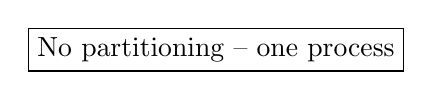
\begin{tikzpicture}
 \pie [ color ={ black!10 , black!50 , black!30 , black!40}, rotate =90, radius=1.5 ]  {47/MAIN, 19/MOM, 34/PRESS}
 \node[draw,align=left] at (0,-3.0) {No partitioning -- one process};
\end{tikzpicture}
\end{minipage}}
\hfil
  \subfigure{
  \begin{minipage}{0.30\textwidth}
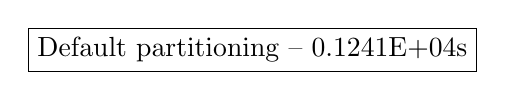
\begin{tikzpicture}
 \pie [ color ={ black!10 , black!50 , black!30 , black!40}, rotate =90, radius=1.5 ]  {50/MAIN, 13/MOM, 37/PRESS}
 \node[draw,align=left] at (0,-3.0) {Default partitioning -- 0.1241E+04s};
\end{tikzpicture}
\end{minipage}}
\hfil
  \subfigure{
  \begin{minipage}{0.30\textwidth}
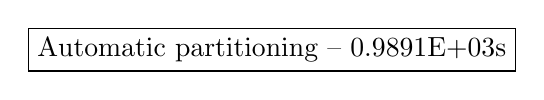
\begin{tikzpicture}
 \pie [ color ={ black!10 , black!50 , black!30 , black!40}, rotate =90, radius=1.5 ]  {64/MAIN, 12/MOM, 24/PRESS}
 \node[draw,align=left] at (0,-3.0) {Automatic partitioning -- 0.9891E+03s};
\end{tikzpicture}
\end{minipage}}
\caption{Distribution of wall-clock time for one and eight processes, solving for an analytic solution, using the default data partitioning for matrix assembly and automatic partitioning to balance the load. MAIN refers to the flux calculation and matrix assembly, MOM to the solution of the linear systems for the momentum balance and PRESS to the solution of the linear systems for the pressure correction.}
\label{fig:distseg}
\end{figure}

\begin{figure}
\begin{tikzpicture}
 \pie [ color ={ black!10 , black!50 , black!30 , black!40}, rotate =90, radius=1.5 ]  {11/MAIN, 89/MOMENTUM+PRESSURE}
\end{tikzpicture}
\caption{Distribution of wall-clock time spent to solve for an analytic solution with the coupled solution algorithm on one processor}
\label{fig:barbalance}
\end{figure}

